\documentclass[conference]{IEEEtran}
\IEEEoverridecommandlockouts
\usepackage{cite}
\usepackage{amsmath,amssymb,amsfonts}
\usepackage{algorithmic}
\usepackage{hyperref}
\usepackage{graphicx}
\usepackage{svg}
\usepackage{textcomp}
\usepackage{xcolor}
\usepackage{multirow}
\usepackage{multicol}
\usepackage{subcaption}
\def\BibTeX{{\rm B\kern-.05em{\sc i\kern-.025em b}\kern-.08em
    T\kern-.1667em\lower.7ex\hbox{E}\kern-.125emX}}
\begin{document}

\title{Parallelized Form Factor Generation for Modeling Diffuse Radiosity}

\author{\IEEEauthorblockN{Eleanor Olson}\email{olsonk@rpi.edu}
\and
\IEEEauthorblockN{Kajsa Arnold}\email{arnolk@rpi.edu}
}
\maketitle
\begin{abstract}
The radiosity technique is an effective method for simulating the diffuse propagation of light in 3D computer graphics rendering. However, it is an expensive calculation, in large part due to the need to calculate form factors for the light transmitted between every pair of faces in a scene. We present a parallel implementation of an algorithm to generate form factors, making use of CUDA, MPI, and MPI I/O. Our implementation performs the basic form factor calculations for diffuse surfaces, then provides corrections for non-convex objects using Monte Carlo simulation techniques. We provide a performance study on the AiMOS supercomputer investigating strong scaling, weak scaling, and the runtime contributions of various parts of the algorithm including communication overhead. We find that this parallelized algorithm significantly decreases the time needed to compute form factors, with a speedup of 14.00 for 16 MPI ranks and CUDA devices in a strong scaling study.
\end{abstract}

\section{Overview}
In computer graphics, when rendering diffuse surfaces it is common to use a ``Radiosity" technique to model these surfaces' interactions with light. This technique splits each face into a number of ``patches", and reduces these diffuse interactions to a systems of equation reduction. While radiosity simulation produces high quality results, it is highly computationally intensive. Specifically, it requires calculating ``form factors" representing the amount of light transmitted between any given pair of face ``patches" within the scene. This calculation is an $O(n^2)$ process in the simplest of cases. When a scene is non convex, however, one must account for shadows, further complicating the running time of the algorithm. In this paper, we outline our techniques to leverage MPI, MPI I/O, and CUDA to create a parallel system that distributes the workload of generating these form factors for a non convex scene. We describe a simple data storage format that can be effectively written in parallel, and evaluate the algorithm's performance on the AiMOS HPC system. 

In the following section, we will give a brief summary of the ray tracing, radiosity, and form factor generation techniques that are relevant to our implementation. In sections III-IV, we describe our implementation in detail, followed by how to build the program. In sections V-VII, we describe our performance testing process, show our results, and analyze these performance studies. We then finish with a summary of the work completed and provide suggestions for future work.


\section{Background}
\subsection{Ray Tracing}
One of the earliest physically based models to render light distribution comes from Whitted \cite{b10}, which outlines the first ``ray tracing" methods. These methods function by projecting a series of rays from the camera plane, bouncing them off of all objects in the scene, and seeing if those paths eventually result in the ray reaching a light source. While this method transformed the field of physically-based rendering, it proved difficult to render a number of physical phenomena with the method. One area in which Whitted Ray Tracing particularly struggles is in rendering the interactions of diffuse surfaces. These surfaces scatter light relatively evenly in all directions, as opposed to non-diffuse surfaces which reflect light uniformly in specific directions. Diffuse surfaces produce a number of unique effects, chief among these being ``color bleeding". This is when a colored area of the scene will gently emit its own color back throughout the room. While this effect is theoretically possible through ray tracing, it is infeasible to send the rays required throughout the scene. Thus, new models needed to be developed.

\subsection{Radiosity}
The first method to effectively model these diffuse surfaces came from Goral, Torrance, Greenberg, and Battaile \cite{b1}. In their solution, they imagined splitting each face within a scene into a number of disparate ``patches". Each of these patches could then calculate what percentage of their own light would escape to any other given patch within the scene. That way, any emissive patches could distribute their light, which in turn would continue to distribute throughout the scene until reaching equilibrium. These ratios of dispersed light between patches are called form factors. Given these form factors, we can express the incoming light at any patch $p_i$ as 
\[ 
R_i = E_i + \rho \sum \limits_{j=0}^{N} R_i F_{ji},
\]
where $R_i$ is the radiosity at $i$, $E_i$ is the emmittence at $i$, and $\rho$ is the reflectance of the patch. The radiosity from each patch is multiplied by the form factor $F_{ji}$ determining how much of the radiation from $j$ will ``reach" $i$. This, when vectorized for all $i$, can then be expressed as solving a system of equations as follows:
\[
\begin{bmatrix}
1-\rho_1 F_{1,1} & -\rho_1F_{1,2} & \cdots & -\rho_1F_{1,N}\\
-\rho_2 F_{2,1} & 1-\rho_2F_{2,2} & \cdots & -\rho_2F_{2,N}\\
\vdots & \vdots & \ddots & \vdots\\
-\rho_N F_{N,1} & -\rho_NF_{N,2} & \cdots & 1-\rho_NF_{N,N}\\
\end{bmatrix} \begin{bmatrix}
    R_1 \\ R_2 \\ \vdots \\ R_N
\end{bmatrix} = \begin{bmatrix}
    E_1\\E_2\\\vdots\\E_N
\end{bmatrix}
\]
This representation, however, does come with some drawbacks. One of the primary disadvantages is that the technique can only model Lambertian surfaces. These are surfaces which uniformly distribute light in all directions. While this can effectively approximate many materials, there are many other diffuse surfaces which direct light in some directions more than others, which must be modeled with more complex techniques.

\subsection{Form Factors}
To calculate the form factors required, Goral et. al. \cite{b1} implement an analytical technique. They define the ratio of light as dependent on the area of the surfaces, as well as the angle between them. As such, they are left with the solvable integral:
\[
F_{i,j} = \frac{1}{A_1} \int \limits_{A_i}^{}\int \limits_{A_j}^{}\frac{\cos(\phi_i)\cos(\phi_j)}{\pi r^2} dA_i dA_j
\]
In this calculation, $\cos(\phi_i)$ is the cosine of the angle between patch $i$'s surface normal and the vector between the two surfaces. A visual representation of these quantities can be found in Figure \ref{fig:ff_geometry}.

\begin{figure}
\includesvg[width=0.48\textwidth]{form_factors.svg}
\caption{A geometric interpretation of the quantities present in the equation for the form factor between two patches $i$ and $j$.}
\label{fig:ff_geometry}
\end{figure}

This calculation works in some cases, however, it severely limits the systems they are able to represent. For instance, the analytical approach to calculating form factors is unable to account for any patch occlusion. Therefore, the scene must be made up of a single, convex mesh. To solve this, a technique of Monte-Carlo simulation can be utilized. With this, we can simply pick a point $p_i$ and $p_j$ on each of the respective faces, and calculate the internals of our integral. We then can average these values and redefine our form factor with the simpler expression:
\[
F_{i,j} = \frac{1}{A_i\cdot N\cdot \pi r^2}\sum\limits_{0}^{N} \cos(\phi_i)\cos(\phi_j)
\]
In this Monte-Carlo approach, our $\cos(\phi_i)$ and $\cos(\phi_j)$ is again compared with the surface normals, but the vector between surfaces is generated either with random sampling or some sort of sampling algorithm.
This alone, however, does not account for any sort of occlusion. The same Monte-Carlo technique, however, may be employed to account for this. One may simply cast some rays, employing a similar technique to \cite{b10} and \cite{b9}, and check which percentage of them are occluded by another face. These Monte-Carlo techniques are the system we employ in our own calculation of form factors.
\section{Implementation}
Our implementation takes advantage of both MPI and CUDA to execute instructions in parallel. Each MPI rank utilizes one CUDA device, and the faces in the scene are split among the MPI rank/CUDA device pairings, so that each rank/device pair is responsible for calculating the same number of form factors. For a visualization of how MPI and CUDA are structured in an example scenario, see Figure \ref{fig:division}.

The program takes in a modified $.obj$ file, which allows for material data to be attached to faces. While this is not useful in form factor calculation, it is critical for solving radiosity overall. Once form factors are generated, they are written to an output `formfactors' file. This is a binary file whose first 4 bytes represent the dimension of the following matrix. This must be a square matrix, and therefore only 1 value is required. The rest of the file is simply a series of 64 bit floating point values, where the $i$'th value corresponds to $F_{i\%N, \lfloor i/N\rfloor}$.

\begin{figure}
\includesvg[width=0.48\textwidth]{division.svg}
\caption{An example diagram showing the interactions between CPU cores and GPUs and what parts of the problem they compute for $s=4$ MPI ranks/CUDA devices and $16$ total patches.}
\label{fig:division}
\end{figure}

When run, the program first initializes all MPI processes, each of which individually read in the mesh. This is done by each process individually, as passing the full input mesh from one process to the rest would induce more latency than each of them processing the mesh in parallel. This is not done with parallelized MPI I/O, as each process must read all data. Once this mesh is read in, we then subdivide according to a user input. This is now the complete mesh we must perform form factor calculation on. We additionally initialize a parallel MPI I/O file to output our final form factors in parallel.

Now that each individual MPI process has a full understanding of the mesh, the calculation of form factors is divided between each MPI process. The form factor calculations for radiosity entering patch $i$ is performed on rank $i\% s$, where $s$ is the number of MPI processes. This iterative system allows us to evenly balance form factor generation between the processes. Since calculating each patch's form factors is a similarly computational complex task to any other patch's form factor calculation, this balance effectively distributes the load, and as such a queuing system is not required. Once the form factors for this are calculated, they can be written directly in parallel into our `formfactors' output file. Given a form factor $F_{i,j}$ we will write to the index in the file $i\cdot N + j$.

Calculation of these form factors is done in a hybrid approach on both the CPU and GPU. The first pass of calculating form factors without accounting for occlusion is done on the GPU. First, given some face $i$ and $j$, we calculate $k$ sample points on each, creating $k$ pairs of positions between them. This array is then added to an input data structure, along with the surface normals ($\vec{n}_i, \vec{n}_j$) of the two faces. This data structure may then be passed into our CUDA functions.

This CUDA implementation, however, must first move this memory into somewhere that the GPU can access. To do so, we utilize CUDA's $\texttt{cudaMallocManaged}$ operation. We allocate an identically sized input array containing the normals and test pairs as well as an $N$ sized array for our output. The input data from the CPU can then be copied into this new input array, and then we may run our CUDA kernel (function). This kernel allocates $N$ blocks (1 per compared face) and $k$ threads per block, allowing each thread to simply perform 1 sample. Each thread then takes the pair of test points $p_i, p_j$ and the normals $\vec{n}_i, \vec{n}_j$, and outputs:
\[
f_{i,j,k} = \left|\frac{(p_i-p_j \cdot \vec{n}_i)(p_j-p_i \cdot \vec{n}_j)}{||p_i-p_j||^2}\right|
\]
Each of these threads can then be reduced on the GPU to sum up to a single value, which can ultimately be averaged to calculate our final form factor. To reduce on the GPU we used sequential thread index based reduction to achieve an $O(n\log n)$ reduction complexity. The array of these averages, then, is returned into the CPU. 

Since the CUDA implementation does not have any knowledge of the underlying mesh, however, it is not able to complete the form factor calculation. First, the CPU must divide each form factor by $A_i$, and then we must calculate occlusion between the form factors. Similarly to our initial computation, we generate $k_2$ sample points $p_i, p_j$ on each face, where $k_2$ is the number of shadow samples we wish to use. We then cast a ray from $p_i$ along the vector $\overline{p_i \to p_j}$, and check its length. If the length is less than the distance between the two points, we know that the cast hit something before reaching its target, and therefore was occluded. We then calculate what proportion of shadow rays were occluded, and multiply that proportion by our original form factor.

These form factors, however, must be normalized. We know that each patch can only emit $1.0\cdot E_i$, and therefore the sum of all form factors along the rows must sum to $1$. To normalize these, we simply sum over all form factor values and divide each by the total. This can then be written to the output file.

Finally, we add a $\texttt{MPI\_Barrier}$ call to synchronize all independent processes before closing our parallel file. We then return the time taken across the entire execution, as well as the total time spent in I/O. This I/O output, however, is the time taken in 1 process, and as such in analysis we multiply this by the number of processes running.

This complete `formfactor' file can then be inputted into a separate program, which uses it to perform matrix reduction and ultimately render it to the screen. An result of this rendering can be seen in Figure \ref{fig:radiosity}.
\begin{figure}
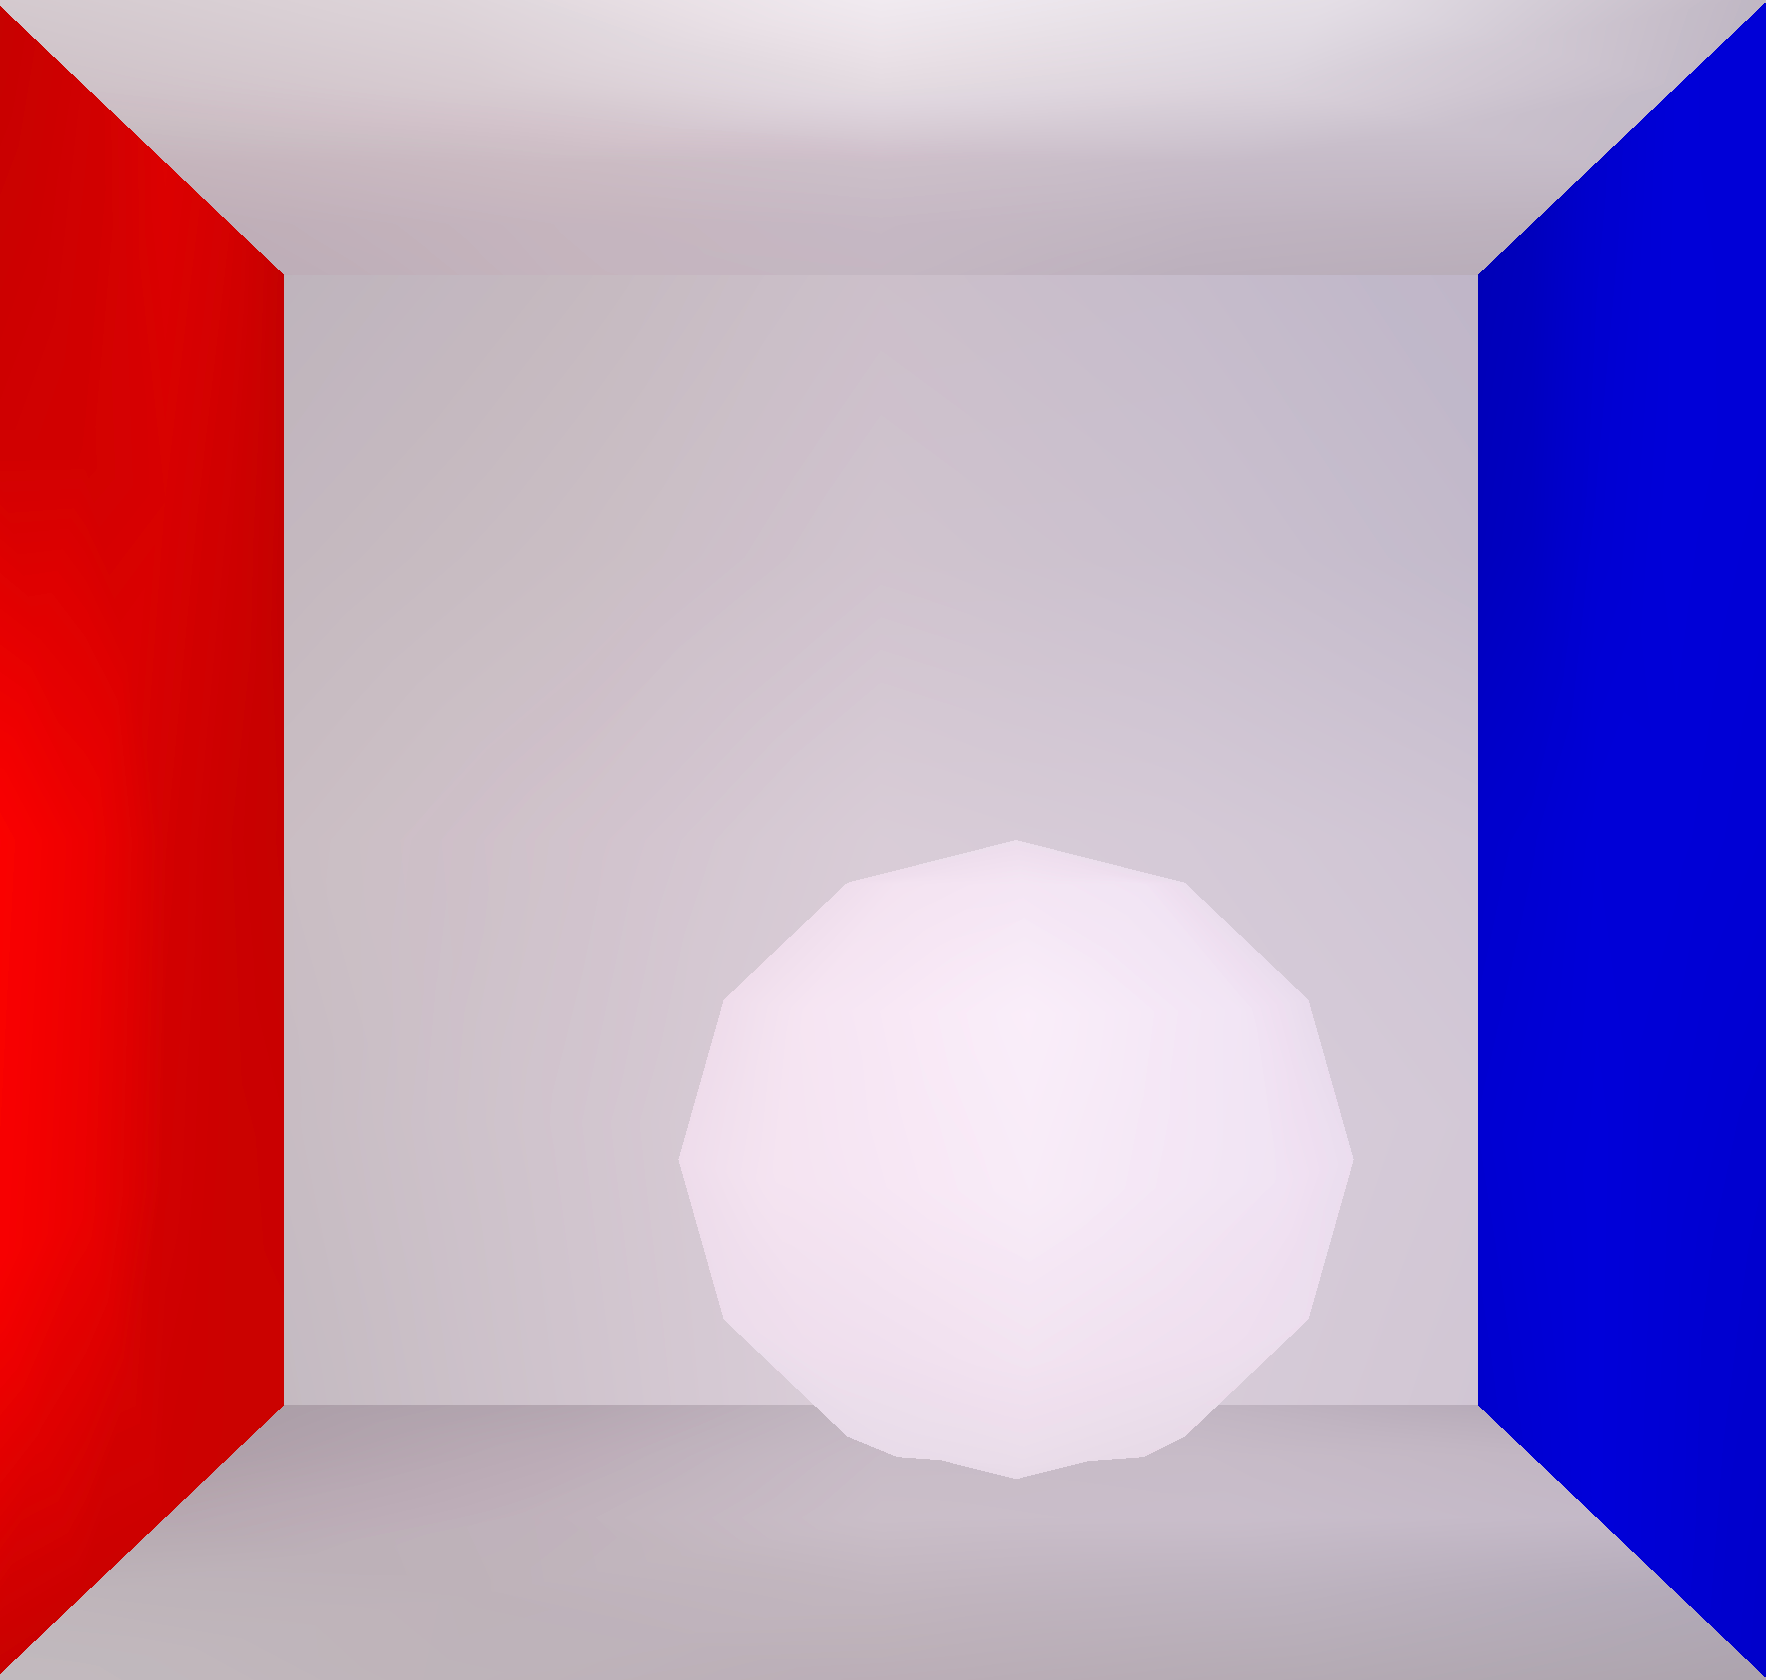
\includegraphics[width=0.48\textwidth]{radiosity.png}
\caption{An example of the output of a full radiosity simulation. This particular input is the same as used to generate form factors in our analysis.}
\label{fig:radiosity}
\end{figure}

\begin{figure*}
\centering
\begin{tabular}{|l|l|ll|ll|ll|ll|}
\hline
\multirow{2}{*}{Processes} & \multicolumn{1}{c|}{Total} & \multicolumn{2}{c|}{I/O}               & \multicolumn{2}{c|}{CUDA Memory}         & \multicolumn{2}{c|}{CUDA Compute}       & \multicolumn{2}{c|}{Occlusion}            \\ \cline{2-10} 
                           & Ticks                      & \multicolumn{1}{l|}{Ticks}   & Percent & \multicolumn{1}{l|}{Ticks}     & Percent & \multicolumn{1}{l|}{Ticks}    & Percent & \multicolumn{1}{l|}{Ticks}      & Percent \\ \hline
1                          & 3127108800                 & \multicolumn{1}{l|}{7667225} & 0.25\%  & \multicolumn{1}{l|}{152092506} & 4.86\%  & \multicolumn{1}{l|}{14414321} & 0.46\%  & \multicolumn{1}{l|}{1364411373} & 43.63\% \\ \hline
4                          & 1794403317                 & \multicolumn{1}{l|}{196626}  & 0.04\%  & \multicolumn{1}{l|}{183979049} & 10.25\% & \multicolumn{1}{l|}{9933998}  & 0.55\%  & \multicolumn{1}{l|}{752554687}  & 41.94\% \\ \hline
16                         & 2784955095                 & \multicolumn{1}{l|}{14400}   & 0.01\%  & \multicolumn{1}{l|}{474591553} & 17.04\% & \multicolumn{1}{l|}{11304810} & 0.41\%  & \multicolumn{1}{l|}{928229786}  & 33.33\% \\ \hline
\end{tabular}
\caption{The number of ticks and percent of the total workload for the weakly scaled study by number of processes. The tick count for both total and I/O ticks are based on a 512MHz processor, and thus represent $1.95\cdot 10^{-9}$ seconds each.}
\label{fig:weaktable_ticks}
\end{figure*}
\vspace{0.05in}
\begin{figure*}
\begin{tabular}{|l|l|ll|ll|ll|ll|}
\hline
\multirow{2}{*}{Processes} & \multicolumn{1}{c|}{Total} & \multicolumn{2}{c|}{I/O}                 & \multicolumn{2}{c|}{CUDA Memory}          & \multicolumn{2}{c|}{CUDA Compute}         & \multicolumn{2}{c|}{Occlusion}              \\ \cline{2-10} 
                           & Ticks                      & \multicolumn{1}{l|}{Ticks}     & Percent & \multicolumn{1}{l|}{Ticks}      & Percent & \multicolumn{1}{l|}{Ticks}      & Percent & \multicolumn{1}{l|}{Ticks}        & Percent \\ \hline
1                          & 256682089250               & \multicolumn{1}{l|}{648184895} & 0.25\%  & \multicolumn{1}{l|}{4672213261} & 1.82\%  & \multicolumn{1}{l|}{2345731044} & 0.91\%  & \multicolumn{1}{l|}{121722999897} & 47.42\% \\ \hline
2                          & 136126952047               & \multicolumn{1}{l|}{68490121}  & 0.10\%  & \multicolumn{1}{l|}{2492728932} & 1.83\%  & \multicolumn{1}{l|}{996610991}  & 0.73\%  & \multicolumn{1}{l|}{68860337312}  & 50.59\% \\ \hline
4                          & 65898566545                & \multicolumn{1}{l|}{8548384}   & 0.05\%  & \multicolumn{1}{l|}{1326360593} & 2.01\%  & \multicolumn{1}{l|}{481395704}  & 0.73\%  & \multicolumn{1}{l|}{32046953812}  & 48.63\% \\ \hline
8                          & 34101875150                & \multicolumn{1}{l|}{1060049}   & 0.02\%  & \multicolumn{1}{l|}{818728502}  & 2.40\%  & \multicolumn{1}{l|}{249593702}  & 0.73\%  & \multicolumn{1}{l|}{16936592193}  & 49.66\% \\ \hline
16                         & 18325372008                & \multicolumn{1}{l|}{188882}    & 0.02\%  & \multicolumn{1}{l|}{743159643}  & 4.06\%  & \multicolumn{1}{l|}{140764006}  & 0.77\%  & \multicolumn{1}{l|}{8080029784}   & 44.09\% \\ \hline
\end{tabular}
\caption{The number of ticks and percent of the total workload for the strongly scaled study by number of processes. The tick count for both total and I/O ticks are based on a 512MHz processor, and thus represent $1.95\cdot 10^{-9}$ seconds each.}
\label{fig:strongtable_ticks}
\end{figure*}
\begin{figure*}
\begin{subfigure}{.49\textwidth}
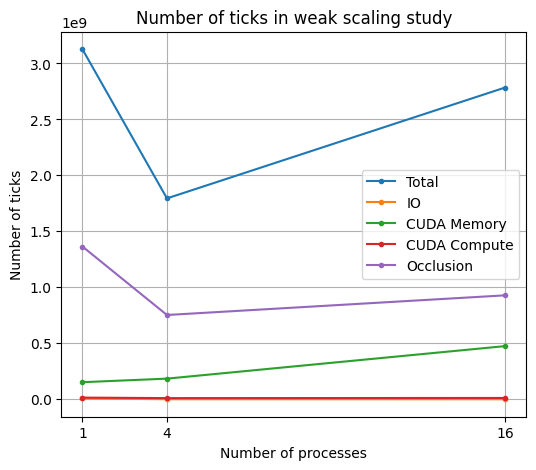
\includegraphics[width=\columnwidth]{ticks_weak.png}
\caption{Weak scaling study}
\label{fig:weakgraph_ticks}
\end{subfigure}
\hspace{0.01\textwidth}
\begin{subfigure}{.49\textwidth}
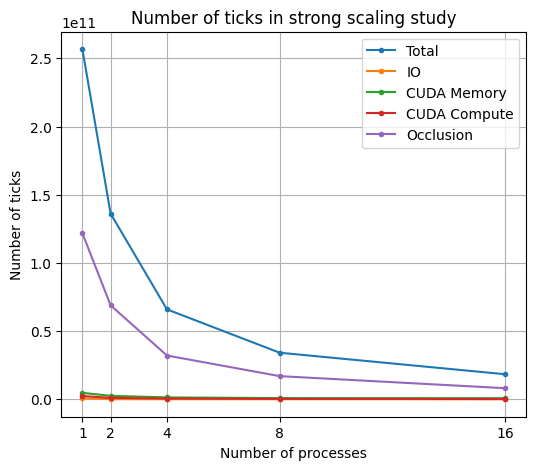
\includegraphics[width=\columnwidth]{ticks_strong.png}
\caption{Strong scaling study}
\label{fig:stronggraph_ticks}
\end{subfigure}
\caption{Graphs of the number of ticks by part of the algorithm for form factor generation.}

\end{figure*}



\section{Building and Running the Simulation}
This simulation was built in C++ using CMake to compile and link the code. To build this simulation, if running on AiMOS, first load the required modules. This can be done with 
$\texttt{module load spectrum-mpi cuda/11.2}$. Then, create a new build directory and run $\texttt{cmake [Solver Source Directory Location]}$. Once CMake has initialized, one can simply run $\texttt{make}$ to generate the outputted $radiosity$ file. This file can be run with the syntax $\texttt{mpirun -n [Number of MPI Processes]}$ $\texttt{./radiosity --input [Input Obj File Reference]}$ $\texttt{--subdiv [Number of Subdivisions]}$. A shell file is available in the publicly available \href{https://github.com/eleanormally/parallel-radiosity}{GitHub} repository for use with the AiMOS slurm scheduler.



\begin{figure*}
\begin{subfigure}{.49\textwidth}
\begin{tabular}{|l|lllll|}
\hline
\multirow{2}{*}{Procs.} & \multicolumn{5}{c|}{Speedup}                                                                                                                                                                                                      \\ \cline{2-6} 
                        & \multicolumn{1}{l|}{Total} & \multicolumn{1}{l|}{I/O}    & \multicolumn{1}{l|}{\begin{tabular}[c]{@{}l@{}}CUDA \\ Mem.\end{tabular}} & \multicolumn{1}{l|}{\begin{tabular}[c]{@{}l@{}}CUDA \\ Compute\end{tabular}} & Occlusion \\ \hline
1                       & \multicolumn{1}{l|}{1.0}   & \multicolumn{1}{l|}{1.0}    & \multicolumn{1}{l|}{1.0}                                                    & \multicolumn{1}{l|}{1.0}                                                     & 1.0       \\ \hline
4                       & \multicolumn{1}{l|}{1.74}  & \multicolumn{1}{l|}{38.99}  & \multicolumn{1}{l|}{0.83}                                                   & \multicolumn{1}{l|}{1.45}                                                    & 1.81      \\ \hline
16                      & \multicolumn{1}{l|}{1.12}  & \multicolumn{1}{l|}{532.44} & \multicolumn{1}{l|}{0.32}                                                   & \multicolumn{1}{l|}{1.28}                                                    & 1.47      \\ \hline
\end{tabular}
\caption{Speedup for weak scaling study.}
\label{fig:weaktable_speedup}
\end{subfigure}
\hspace{0.01\textwidth}
\begin{subfigure}{0.49\textwidth}
\begin{tabular}{|l|lllll|}
\hline
\multirow{2}{*}{Procs.} & \multicolumn{5}{c|}{Speedup}                                                                                                                                                                                                       \\ \cline{2-6} 
                        & \multicolumn{1}{l|}{Total} & \multicolumn{1}{l|}{I/O}     & \multicolumn{1}{l|}{\begin{tabular}[c]{@{}l@{}}CUDA \\ Mem.\end{tabular}} & \multicolumn{1}{l|}{\begin{tabular}[c]{@{}l@{}}CUDA \\ Compute\end{tabular}} & Occlusion \\ \hline
1                       & \multicolumn{1}{l|}{1.0}   & \multicolumn{1}{l|}{1.0}     & \multicolumn{1}{l|}{1.0}                                                    & \multicolumn{1}{l|}{1.0}                                                     & 1.0       \\ \hline
2                       & \multicolumn{1}{l|}{1.89}  & \multicolumn{1}{l|}{9.46}    & \multicolumn{1}{l|}{1.87}                                                   & \multicolumn{1}{l|}{2.35}                                                    & 1.77      \\ \hline
4                       & \multicolumn{1}{l|}{3.90}  & \multicolumn{1}{l|}{75.83}   & \multicolumn{1}{l|}{3.52}                                                   & \multicolumn{1}{l|}{4.87}                                                    & 3.80      \\ \hline
8                       & \multicolumn{1}{l|}{7.53}  & \multicolumn{1}{l|}{611.47}  & \multicolumn{1}{l|}{5.71}                                                   & \multicolumn{1}{l|}{9.40}                                                    & 7.19      \\ \hline
16                      & \multicolumn{1}{l|}{14.01} & \multicolumn{1}{l|}{3431.68} & \multicolumn{1}{l|}{6.29}                                                   & \multicolumn{1}{l|}{16.66}                                                   & 15.06     \\ \hline
\end{tabular}
\caption{Speedup for strong scaling study.}
\label{fig:strongtable_speedup}
\end{subfigure}
\caption{Speedup for the total workload and each part of the algorithm for form factor generation, by number of processes.}

\end{figure*}
\begin{figure*}
\begin{subfigure}{.49\textwidth}
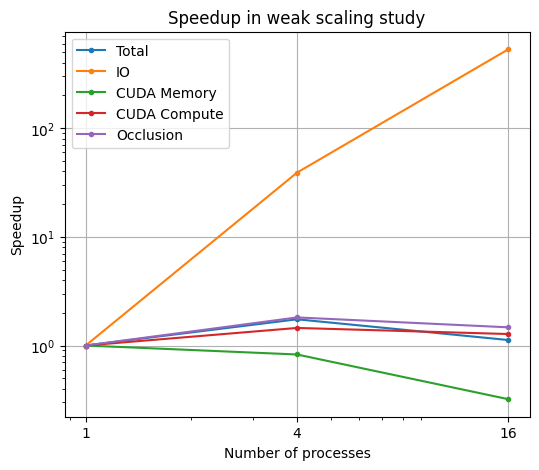
\includegraphics[width=\columnwidth]{weak_new.png}
\caption{Speedup for weak scaling.}
\label{fig:weakgraph_speedup}
\end{subfigure}
\hspace{0.01\textwidth}
\begin{subfigure}{.49\textwidth}
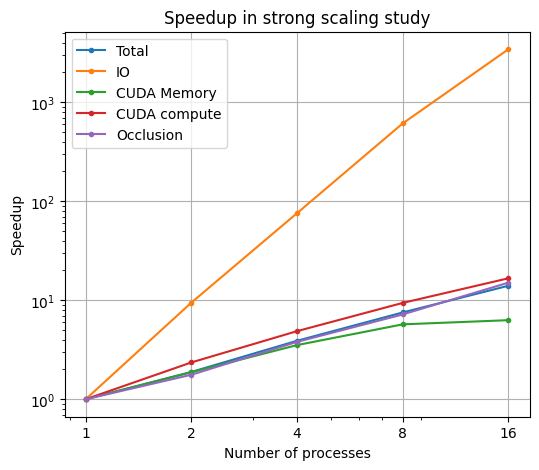
\includegraphics[width=\columnwidth]{strong_new.png}
\caption{Speedup for strong scaling.}
\label{fig:stronggraph_speedup}
\end{subfigure}
\caption{Graphs of the speedup by part of the algorithm for form factor generation.}
\end{figure*}


\section{Testing Form Factor Generation}
We ran and tested this code on the RPI AiMOS supercomputer. Specifically, we tested on the $el8-rpi$ cluster, providing us with nodes containing 2x 20 core POWER9 processors and 4 NVidia Volta V100 GPUs. 
Our tests were performed with an input similar to the standard "Cornell Box" \cite{b1} with an added sphere in the center to create occlusion. The base mesh had 46 faces, and uses 512 samples between each face to calculate form factors. Additionally, each form factor casts 32 shadow samples to measure occlusion.

\section{Results}
We analyzed our performance scaling in both strong and weak scaling contexts. While analyzing strong scaling performance is naturally intuitive in form factor generation, it is more difficult to create an environment that weakly scales for this category of compute. To create an input which will scale proportionally to the number of processors, we decided to subdivide each face. This multiplies the total number of patches by 4 with each subdivision, allowing us to multiply the process count by 4 to scale with it. While these subdivisions allow us to analyze our method's weak scaling performance, they come with the drawback of limiting our possible weak-scaled process counts to numbers of the form $4^s$, where $s$ is the number of subdivisions performed on the input mesh. Due to resource constraints, we tested weak scaling performance on a maximum of 4 nodes, allowing for a total of 16 simultaneous processes using distinct GPUs. The timing results are shown in Figures \ref{fig:weaktable_ticks} and \ref{fig:weakgraph_ticks}, and the speedup calculations are shown in Figures \ref{fig:weaktable_speedup} and \ref{fig:weakgraph_speedup}.

To analyze strong scaling, we used the same ``Cornell Box" with a sphere input mesh, and subdivided it 3 times for each test. This created a total of $2944$ patches requiring form factors. Since, unlike weak scaling, strong scaling does not restrict the number of processes we may test with, we then analyzed performance for all $2^n$ processor counts from $0\leq n \leq 4$. These results are shown in Figures \ref{fig:strongtable_ticks} and \ref{fig:stronggraph_ticks}, and the speedup calculations in Figures \ref{fig:strongtable_speedup} and \ref{fig:stronggraph_speedup}.


In addition to recording the total time to complete the simulation, we also timed specific parts of the algorithm to gain insight into their performance impact on the program as a whole. The I/O time describes the time to perform MPI I/O operations, which occurs when each rank writes the form factor output to a file. The CUDA memory time is the time taken to copy the sample point pairs into an array that is accessible on the GPU. The CUDA compute time is the time spent in the CUDA kernel, which calculates the line factor for each pair of points and performs a block reduction. Finally, the occlusion time is the time to perform the second stage of form factor calculation that is performed on the CPU, which deals with shadow rays that decrease the value of the form factors.  

\section{Analysis}
\subsection{Strong Scaling}
Considering the strong scaling study, we see an approximately linear relationship between number of processes and overall speedup, with a coefficient multiplier of 1. This indicates that the added complexity of initializing MPI I/O as well as communicating between the CPU and GPU is insignificant compared to the benefit of splitting up the calculation of the form factor for each individual patch.  At 16 processes, we begin to see a slight drop in total speedup compared to the expected linear relationship; at 16 processes, the speedup over a serial implementation is approximately 14. Based on the speedup graph in Figure \ref{fig:stronggraph_speedup}, the factor that most likely has the largest contribution to this is the CUDA memory copy portion of the program. From 1 to 8 processes, the memory copy portion scales approximately linearly with a coefficient of 1.8, it falls short of this number for 16 processes, and this is a primary contributor to the decrease in speedup overall. Since parts of the $\texttt{cudaMallocManaged}$ function are executed serially per node, it makes sense that we would start to see decreased performance from this part of the program as we reach processor counts that require more than one node. 

Considering other individual parts of the simulation in the strong scaling study, we see that both the CUDA compute and occlusion portions scale linearly with a similar coefficient to the overall program. An exception is the I/O portion, which scales exponentially with the number of ranks/processes. For a strong scaling study, an increase in the number of ranks means that each rank is writing fewer form factors to the file, and so more writes are performed in parallel. The exponential speedup relationship indicates that this is a very significant optimization compared to writing to the file serially, justifying the use of MPI I/O.

\subsection{Weak Scaling}
In the weak scaling study, we see a more complex relationship between number of processes and speedup. As shown in Figure \ref{fig:weakgraph_speedup}, the total speedup increases to 1.74 for 4 processes, then drops down to 1.12 for 16 processes. This reflects the presence of some complex competing factors within the program. Since with increased parallelization we do not see a consistent increase or decrease in performance, we cannot solely attribute the relationship to the amount of overhead versus actual computation that is occurring within the parallelized part of the program. One possible explanation is that in going from 4 processes to 16 processes, we are forced to use 4 nodes rather than 1, as the AiMOS cluster used only has 4 GPUs per node. Going from 1 node to 4 nodes increases communication overhead, especially if portions of the network become saturated. In short, we could be experiencing a benefit due to increased parallelization at 4 processes, but have this be negated by communication slowdowns at 16 processes. It would be informative to have more data points for this analysis, but the limitations of this problem prevent us from performing weak scaling analysis on other numbers of processes for reasons described in the previous section.

Turning our attention to the weak scaling results for individual portions of the simulation, we again see that the CUDA compute and occlusion portions scale similarly to the speedup for the program as a whole. The CUDA memory portion consistently decreases in performance as the number of processes increases. This is expected, as an increased overall problem size means that each rank needs to allocate and copy more data. The I/O portion of the program has increasing performance as the number of processes increases. We wouldn't necessarily expect an increase in I/O performance as the number of processes increases in a weak scaling study, but it is important to note that the total amount of time spent in I/O was small. As a result, small amounts of variability will have more of an impact on the speedup values. 

\subsection{Communication Overhead}
In Figures \ref{fig:stronggraph_ticks} and \ref{fig:weakgraph_ticks}, we see the number of ticks taken to complete various sections of the simulation. From this chart, we see that the part of the program that takes the most time is the occlusion calculations (the second part of form factor calculation that takes place in parallel on the CPU). In smaller problem sizes, memory allocation for use on the CUDA devices also becomes a somewhat significant portion of the runtime. The CUDA computation and I/O steps are relatively a very small part of the total runtime. Overall, this indicates that communication overhead is low compared to the amount of time spent doing real computational work. As expected, a larger proportion is spent in communication overhead for smaller problem sizes than for larger ones.

Considering I/O performance specifically, the percentage of the program spent in I/O never exceeded $0.25\%$. The amount of information that needs to be written to a file is small for this problem. The use of parallel I/O through MPI provided significant speedups for the I/O code, but the overall impact on the program is low due to the small amount of data that needs to be written.

\subsection{Hybrid CPU/GPU Compute}
There are two major compute portions to this problem: the basic form factor calculation, which occurs on the GPU, and the occlusion correction, which occurs on the CPU. In a naive serial implementation, the basic form factor calculation is $O(n^2)$ where $n$ is the number of faces, while the occlusion calculation is $O(n^3)$. Each form factor occlusion must perform $n$ form factor calculations, which each must compare $k$ (a constant) samples between $n$ partner faces. The occlusion correct requires similar iteration, however each ray cast must also iterate across all $n$ faces, thus making the process $O(n^3)$. Through parallelization, we can effectively reduce the runtime scaling of form factor generation from $O(n^2)$ to $O(n)$. This is how our current CUDA implementation is written. This, however, is an imperfect measurement of runtime complexity as it ignores the increased time associated with higher memory footprints, which remain $O(n^2)$. 

Because shadow occlusion currently is run on the CPU, we do not see any parallelism time complexity changes. Of course our runtime is divided by the number of MPI processes, but this can be understood as a constant time change, and as such does not modify the underlying time complexity. If we were to parallelize shadows, we could theoretically reduce this time complexity down to $O(n\cdot \log n)$, given that each occlusion form factor could be stored in a block, each face in the ray cast in a thread, and then perform $O(\log n)$ reduction on these to find the closest; however, this is not present in our current implementation.

Overall, due to shadow calculation, our total theoretical runtime remains $O(n^3)$. However, to this section taking up varying percentages of our runtime, as discussed throughout this section, effectively analyzing this kind of scaling remains challenging with our hybrid MPI and CUDA approach.

\section{Conclusion}
\subsection{Summary}
In this paper, we have presented an implementation for computing form factors for diffuse, non-convex surfaces. This approach is parallelized using CUDA, MPI, and MPI I/O. Our performance studies showed that parallelization was indeed effective, with an observed speedup of 14.00 for 16 ranks/devices in our strong scaling study. This is a useful result, as form factors are an expensive part of radiosity calculations used in rendering 3D scenes. Despite the successes of this algorithm, there are areas for improvement in further parallelization. These are described in the following section.  


\subsection{Future Work}
One of the largest areas of future work is in the parallelization of the system of equations reduction. While some papers \cite{b3}, \cite{b4}, \cite{b7} have introduced techniques for this sort of parallelized matrix reduction, this was out of scope for our particular work. This, however, is made significantly more complicated by our use of AiMOS for radiosity solutions. Since the architecture does not have first class support for graphics APIs such as OpenGL or Vulkan, nor does it have somewhere to display these graphics, it is substantially more difficult to generate images directly on the supercomputer. 
Another avenue of work comes in further optimizing the form factor generation. One area of optimization can be seen when reanalyzing the equation for form factors: 
\[
F_{i,j} = \frac{1}{A_1} \int \limits_{A_i}^{}\int \limits_{A_j}^{}\frac{\cos(\phi_i)\cos(\phi_j)}{\pi r^2} dA_i dA_j
\]
We can see that apart for the term $\frac{1}{A_1}$, the form factor for $F_{i,j}$ and $F_{j,i}$ is identical. Therefore, we can simply define $F_{j,i} = \frac{A_i}{A_j}F_{i,j}$, and we only need to calculate the upper corner of the form factor matrix. This, however, introduces difficulties in load balancing. Since later rows are significantly simpler to compute, we must make sure that they are evenly distributed among the processes. This could be done using a queuing system and passing messages between processes; however, this introduces a significant amount of inter process communication and latency to the system. Additionally, this would require each process to send its form factor results back to a central coordinating process, preventing our efficient use of MPI I/O. 

In addition to this optimization, we can turn to optimizing our shadow sampling. As discussed previously, our shadow samples are currently calculated on the CPU. This is because it requires the full mesh to be loaded and compared against, and requires ray casting. While some techniques, such as \cite{b11} have implemented ray casting and ray tracing on programmable graphics hardware, it is a significant challenge that proved out of scope for this project. Doing so, however, would significantly speed up the form factor generation, and would additionally allow for higher shadow sample counts.
\section{Contributions}
This project was done in a group of two. Eleanor's role included coding and running the form factor solver and writing the majority of some paper sections, including the background, implementation, description of the performance testing process, and future directions. Kajsa's contribution included graphs and analysis for the performance studies, work on the introduction and conclusion, and the creation of diagrams for the paper and paper formatting.
\section{Acknowledgments}
The code used to process meshes and cast rays, as well as to visualize the output, is built on the work done by Professor Barbara Cutler for her Advanced Computer Graphics course. This base code was used with permission, and with great thanks to Dr. Cutler for allowing us to build off of this work.
\begin{thebibliography}{00}
\bibitem{b1} C. Goral, K. Torrance, D. Greenberg, and B. Battaile, ``Modeling the interaction of light between diffuse surfaces," SIGGRAPH Comput. Graph, vol. 18, no. 3, pp. 213-222, July 1984.

\bibitem{b2} J. Nasman and J. Zolla, ``Parallel Radiosity Using the Message Passing Interface," Assassin.cs.rpi.edu.

\bibitem{b3} O. Adenikinju, J. Gilyard, J. Massey, T. Stitt, J. S. Graf, X. Huang, S. Khuvis, M. K. Gobbert, Y. Wang, and M. Olano, ``Real time global illumination solutions to the radiosity algorithm using hybrid CPU/GPU nodes," Technical Report HPCF-2014-15, UMBC High Performance Computing Facility, University of Maryland, Baltimore County, 2014.

\bibitem{b4} O. Adenikinju, J. Gilyard, J. Massey, and T. Stitt, ``Concurrent solutions to linear systems using hybrid CPU/GPU nodes," SIAM Undergraduate Research Online (SIURO), 2015.

\bibitem{b5} D. Greenberg, M. Cohen, and K. Torrance, ``Radiosity: a method
for computing global illumination", The Visual Computer, vol. 2, pp.291–297, September 1986.

\bibitem{b6} A. Uejima and K. Yamazaki, ``Parallel radiosity: Evaluation of parallel form factor calculations and a static load balancing algorithm," in \emph{Lecture Notes in Computer Science}, C. Polychronopoulos, K. J. A. Fukuda, and S. Tomita, Eds, vol. 1615. Heidelberg, Berlin, Germany:Springer.

\bibitem{b7} S. M. Drucker and P. Schroder, ``Fast radiosity using a data parallel architecture," May 1992, [Online]. Available: https://www.microsoft.com/en-us/research/publication/fast-radiosity-using-a-data-parallel-architecture/.

\bibitem{b8} M. Cohen, E. Chen, J. Wallace, and D. Greenberg, ``A Progressive Refinement Approach to Fast Radiosity Image Generation," ACM Computer Graphics, vol. 22, no. 4, pp.75–84, 1988.

\bibitem{b9} J. Wallace, K.A. Elmquist, and E. Haines, ``A Raytracing Algorithm for Progressive Radiosity," ACM Computer Graphics, vol. 23, no. 3, pp.315–324, 1989.

\bibitem{b10} T. Whitted, ``An Improved Illumination Model for Shaded Display," Communications of the ACM, vol. 23, no.6, pp.343–3349, 1980.
\bibitem{b11} T. Purcell, I. Buck, W. Mark, and P. Hanrahan, ``Ray Tracing on Programmable Graphics Hardware" ACM Transactions on Graphics, vol. 21, no. 3, pp.703-712, 2002

\end{thebibliography}
\end{document}


%% Weak Scaling

Processes | Total Ticks | IO     | Cuda Memory | Cuda Compute | Shadow  
1         | 3127108800  |7667225 | 152092506   | 14414321     | 1364411373
4         | 1794403317  |3146021 | 183979049   | 9933998      | 752554687
16        | 2784955095  |3686429 | 474591553   | 11304810     | 928229786
%%
%%
Strong Scaling
Processes | Total Ticks | IO        | Cuda Memory | Cuda Compute| Shadow  
1         |256682089250 | 648184895 | 4672213261  | 2345731044  | 121722999897
2         |136126952047 | 273960484 | 2492728932  | 996610991   | 68860337312
4         |65898566545  | 136774146 | 1326360593  | 481395704   | 32046953812
8         |34101875150  | 67843136  | 818728502   | 249593702   | 16936592193
16        |18325372008  | 48353901  | 743159643   | 140764006   | 8080029784

%%